\section{Evaluation and Analysis}

\subsection{Datasets}
\begin{itemize}
\item Beijing
\item Movebank/Starkey
\item Singapore
\end{itemize}

\subsection{Existing Methods and comparisons} 

\paragraph{DTW}
\par Definition and short description
Problems with DTW
\begin{figure}
\centering     
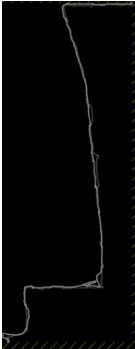
\includegraphics[scale=0.8]{figs/dtw_probs_1_1.jpg}
\caption{Two Trajectories with dissimilarity 250.6}
\label{fig:dtw_prob_1}  
\end{figure} 

\begin{figure}[H]
\centering     
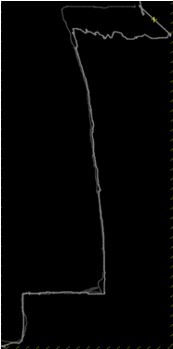
\includegraphics[scale=0.8]{figs/dtw_probs_1_2.jpg}
\caption{Two trajectories with dissimilarity 111.6}
\label{fig:dtw_prob_2}  
\end{figure} 

As shown in \ref{fig:dtw_prob_1} \ref{fig:dtw_prob_2}, two closer trajectories are given higher dissimilarity than the ones which are apart. This is due to the uneven sampling of the trajectories. 

\paragraph{SWARM}
\par Short Description . 
Problems with SWARM 
\begin{itemize}
\item Does not report all the big clusters
\item Dependent a lot on the sample points. If we resample, it would be computationally more expensive than our approach.
\end{itemize}

\paragraph{TrajClus}
\par Short Description 

\subsection{Clustering Effectiveness}

\subsubsection{Silhouette Coefficient}
We show that the proposed algorithm clusters significantly better by using Silhouette Coefficient (SC); a standard metric that shows the effectiveness of clustering. SC is based on the cohesion and the separation of clusters formed. The cohesion ( \textit{a(x)})  is defined as the average distance of x to all other vectors in the same cluster. 
The separation (\textit{b(x)}) is defined as the minimum of the average distances of x to the vectors in other clusters.
Further, the silhouette coefficient of a data point is defined as 
\begin{equation}
s(x)=\frac{b(x)-a(x)}{max(a(x),b(x))}
\end{equation}
The total silhouette coefficient of the dataset is the average over all the points given by
\begin{equation}
SC=\frac{1}{N}\sum_{i=1}^{N}s(x)
\end{equation}
\noindent Ideally, SC is between [-1,1], where values closer to 1 representing better formed clusters. 
Figure~\ref{figs:sil_cdf} shows that our algorithm provides x\%\ldots improvement over SWARM. DTW performs the worst where the clustering \ldots. In more than \rednote{90\%} of the scenarios, OD-based clustering outperforms DTW by \rednote{some percentage}, and outperforms SWARM by \rednote{some percentage}.

\begin{figure}
\centering     
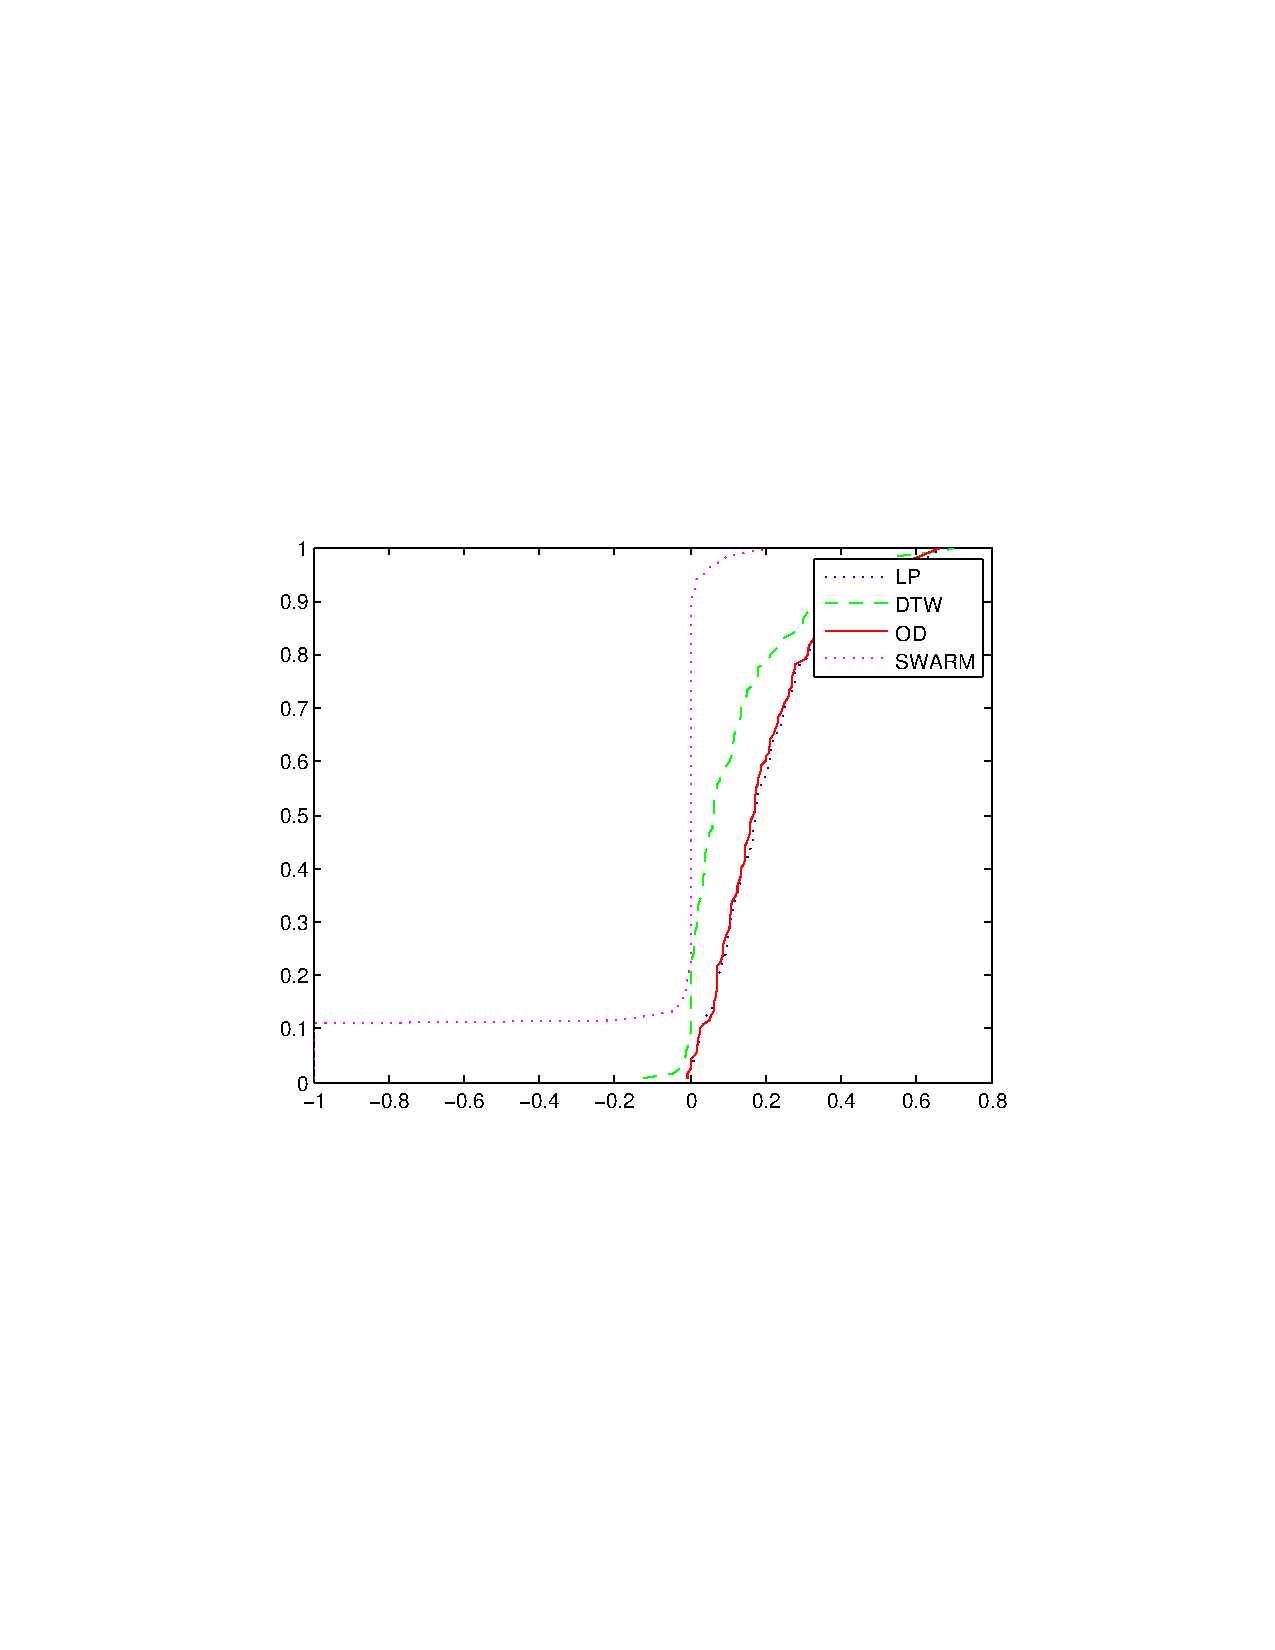
\includegraphics[scale=0.3]{figs/sil_cdf.jpg}
\caption{Comparison of silhouette coefficients for different schemes: OD- and LP-based clustering outperform existing mechanism. We outperform clusters found by DTW by order(s) of magnitude}
\label{fig:sil_cdf}  
\end{figure}

\subsubsection{Analysis of OD-clustering}

\paragraph{Variance in origins and destinations}
Figure~\ref{fig:od_cdf} and \ref{fig:angle_cdf} show that OD- and LP-based clustering schemes have relatively low OD differences.However, DTW and SWARM have very less trajectories per cluster giving rise to low SSW values.  

\begin{figure}
\centering     
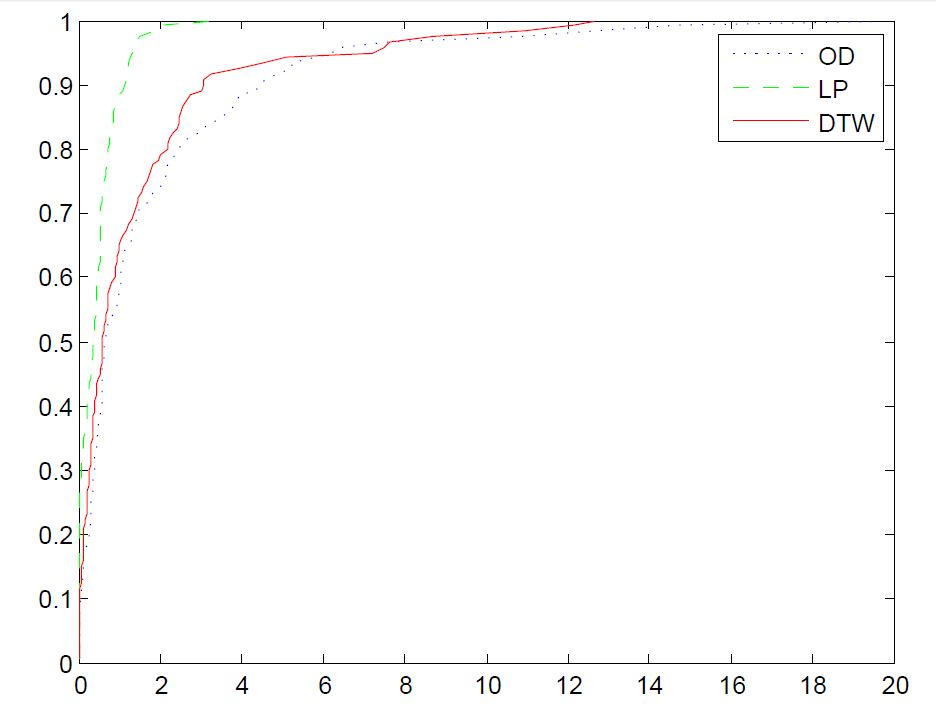
\includegraphics[scale=0.3]{figs/od_cdf.jpg}
\caption{}
\label{fig:od_cdf}  
\end{figure} 

\begin{figure}[H]
\centering     
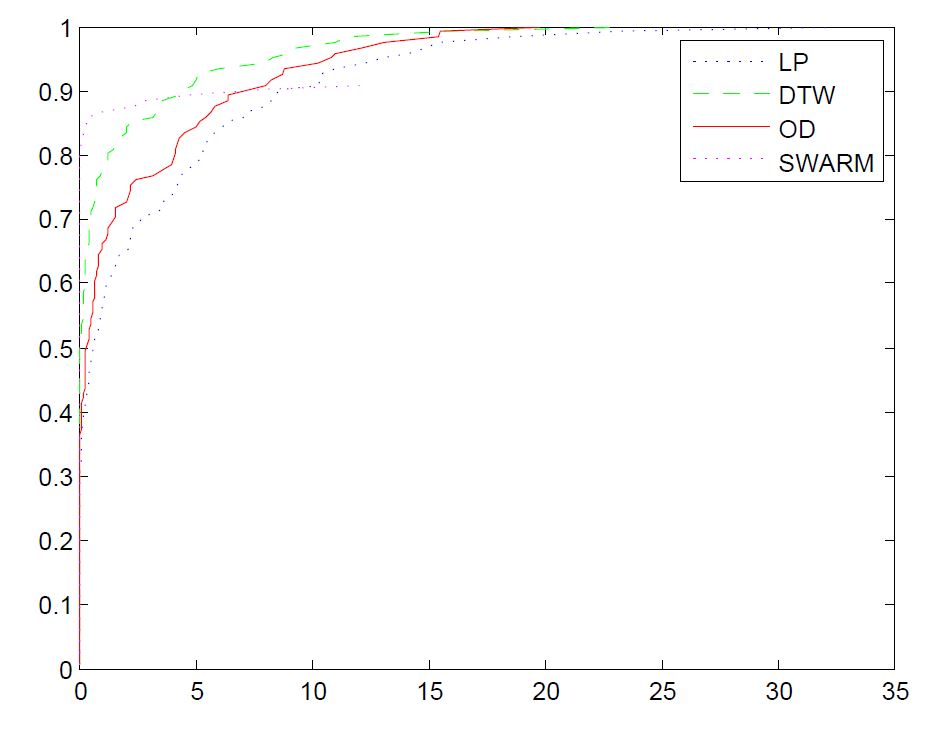
\includegraphics[scale=0.3]{figs/angle_cdf.jpg}
\caption{CDF of angle for optimal cluster for LP-DTW-OD}
\label{fig:angle_cdf}  
\end{figure} 

\subsubsection{Sum of Squares Within Clusters}

(SWARM has very large SSW and OD variance values for some users, which skews the plots. Have Left it out for now, will have to change plots to logscale) 

\begin{figure}[H]
\centering     
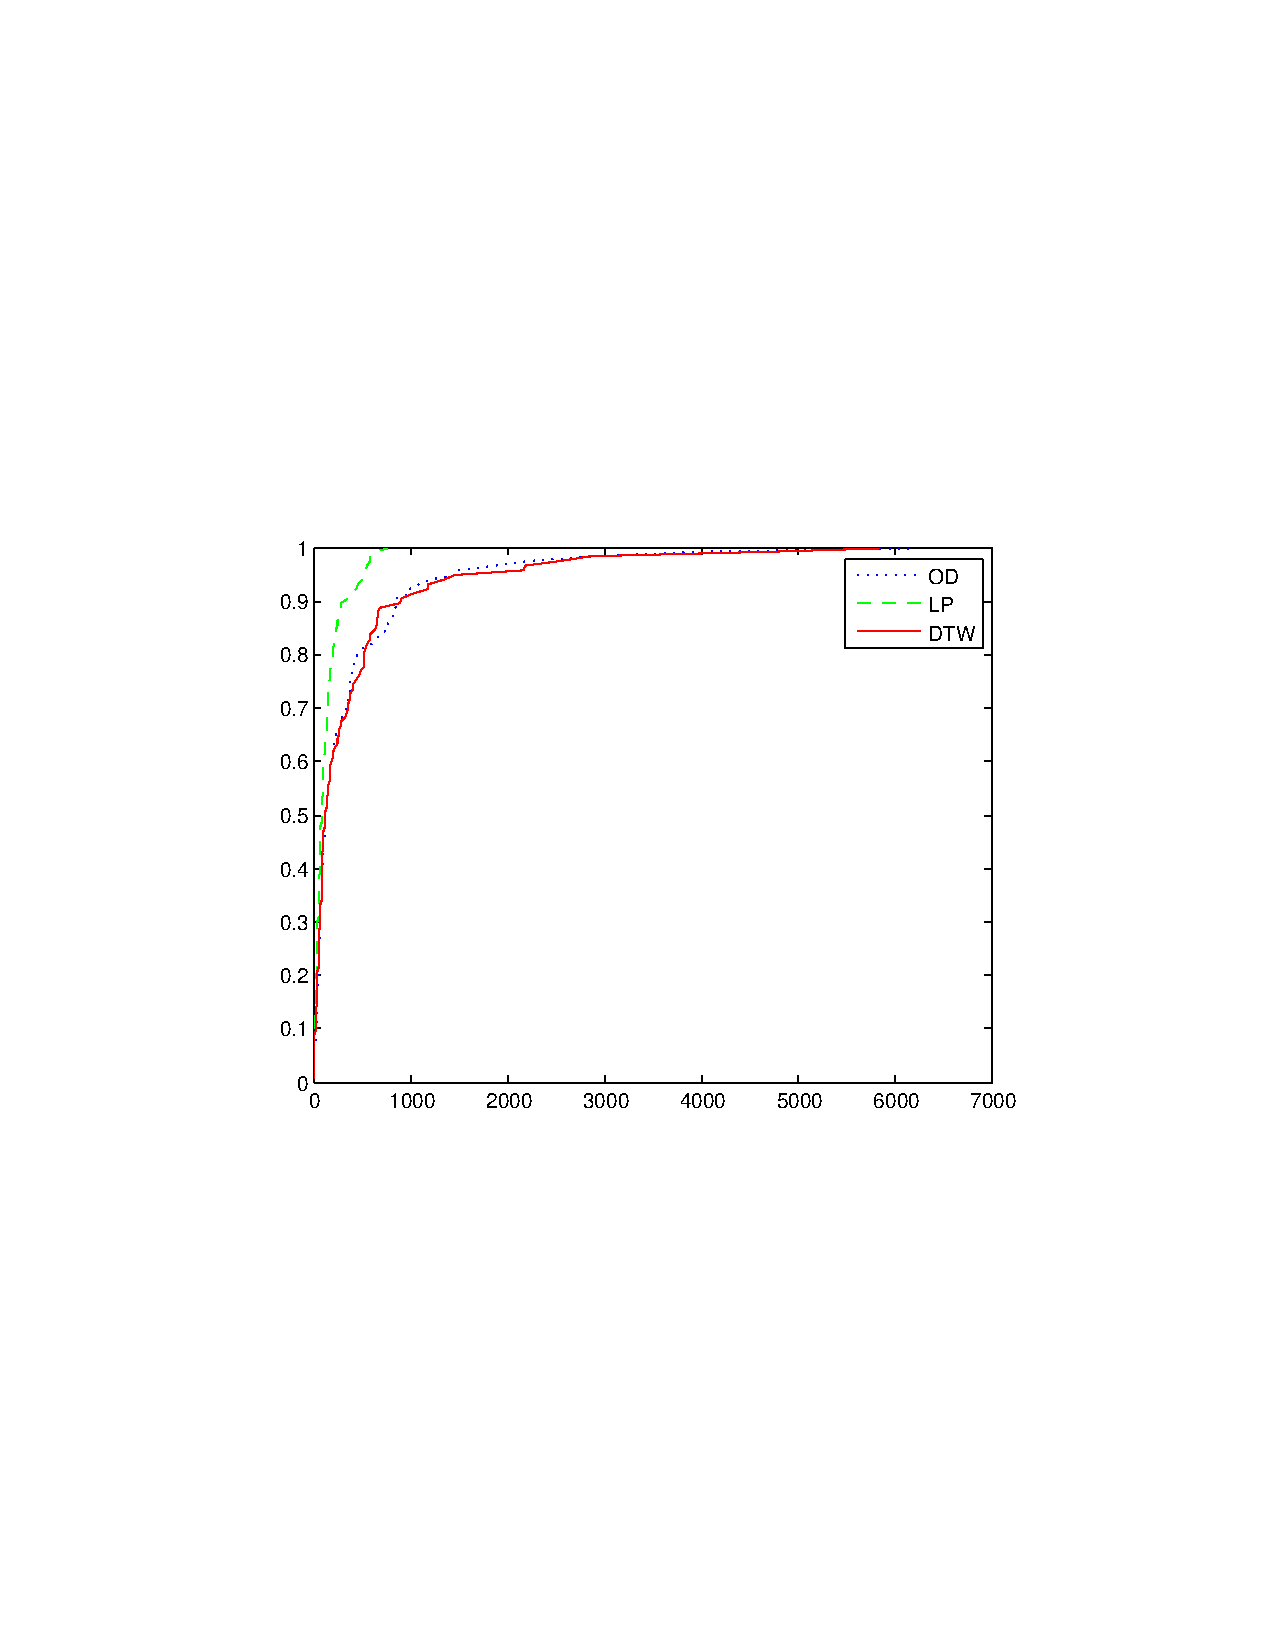
\includegraphics[scale=0.3]{figs/ssw_cdf.jpg}
\caption{CDF of SSW for optimal cluster for LP-DTW-OD}
\label{fig:ssw_cdf}  
\end{figure} 

\paragraph{Definition}
The sum of squares within clusters is defined as
\begin{equation}
SSW=\sum _{i=1}^{n}(\left |x_i-c_i  \right |)^2
\end{equation}
where $x_i$ is a data point and $c_i$ is the mean of the cluster it belongs to. In the case of Trajectory analysis, we consider the pointwise summation of the Haversine distance between the trajectory and the mean trajectory of that cluster, over all the sample points. 

\paragraph{Some Key Points for SSW Curves}
The reason behind the low SSW values for DTW method is that it does not discover all the trajectories in the final clusters. This is because the point in the dendrogram where the condition for reporting final clusters is satisfied, is very low when DTW is used as a similarity metric. 


\subsubsection{Average Trajectories Per Cluster}
Number of clusters with large number of trajectories in it is better (Figure~\ref{fig:avg_cdf} and ~\ref{fig:avgtop_cdf}). Clearly, we summarize a human's movement better.

\begin{figure}[H]
\centering     
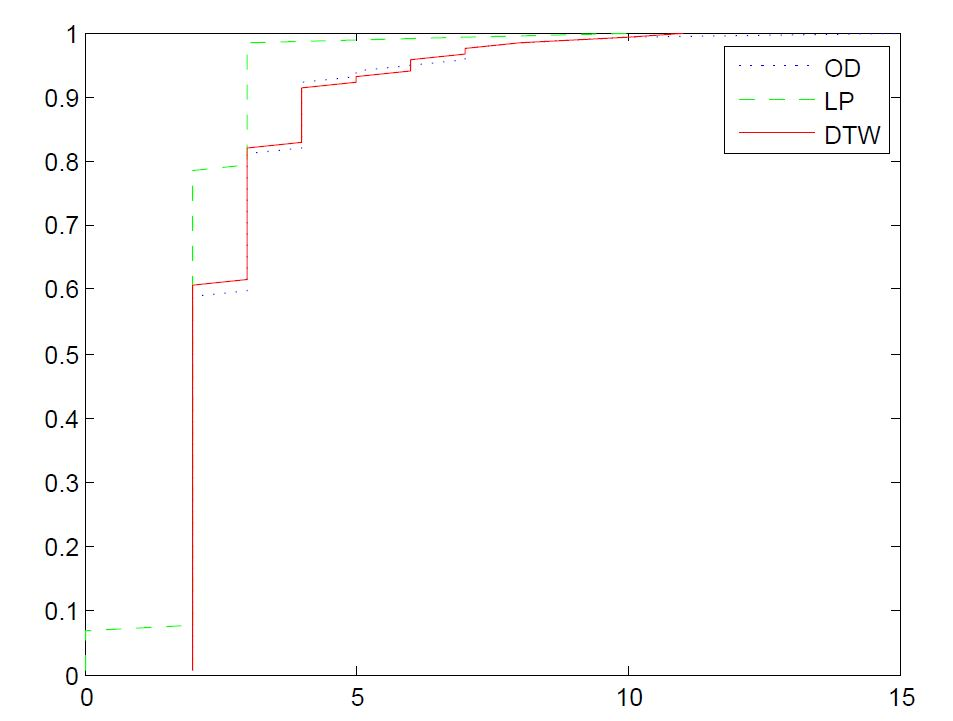
\includegraphics[scale=0.3]{figs/avg_cdf.jpg}
\caption{CDF of average trajectories per cluster for LP-DTW-OD}
\label{fig:avg_cdf}  
\end{figure} 

\begin{figure}[H]
\centering     
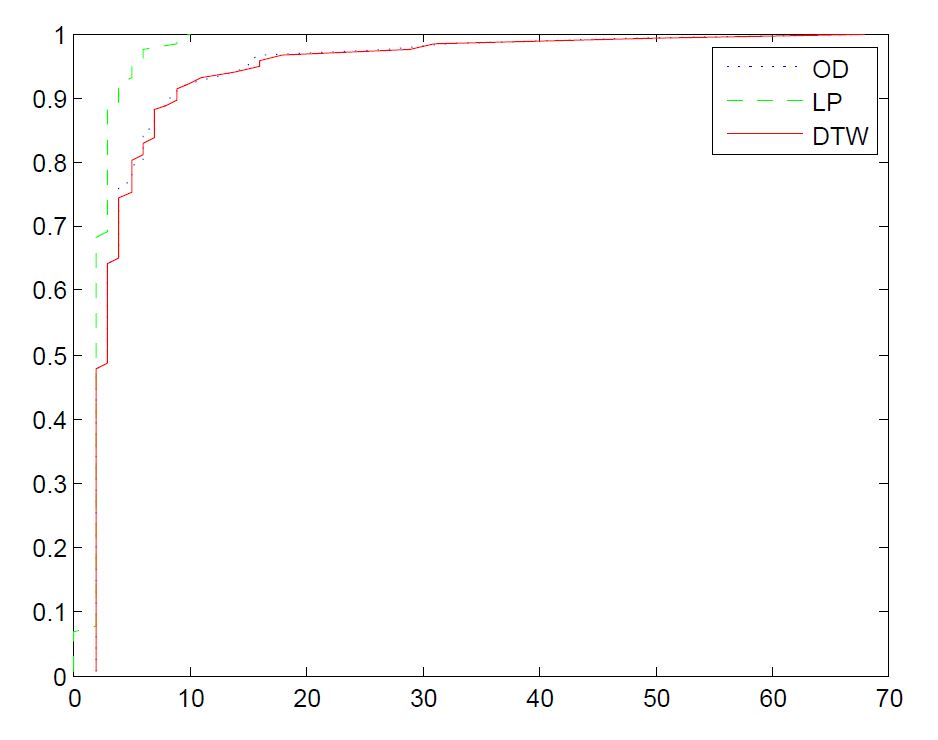
\includegraphics[scale=0.3]{figs/avgtop_cdf.jpg}
\caption{CDF of average trajectories per top-k clusters for LP-DTW-OD}
\label{fig:avgtop_cdf}  
\end{figure} 

\subsection{Computation Time}

\paragraph{Discussion on time complexity }

\begin{figure}[H]
\centering     
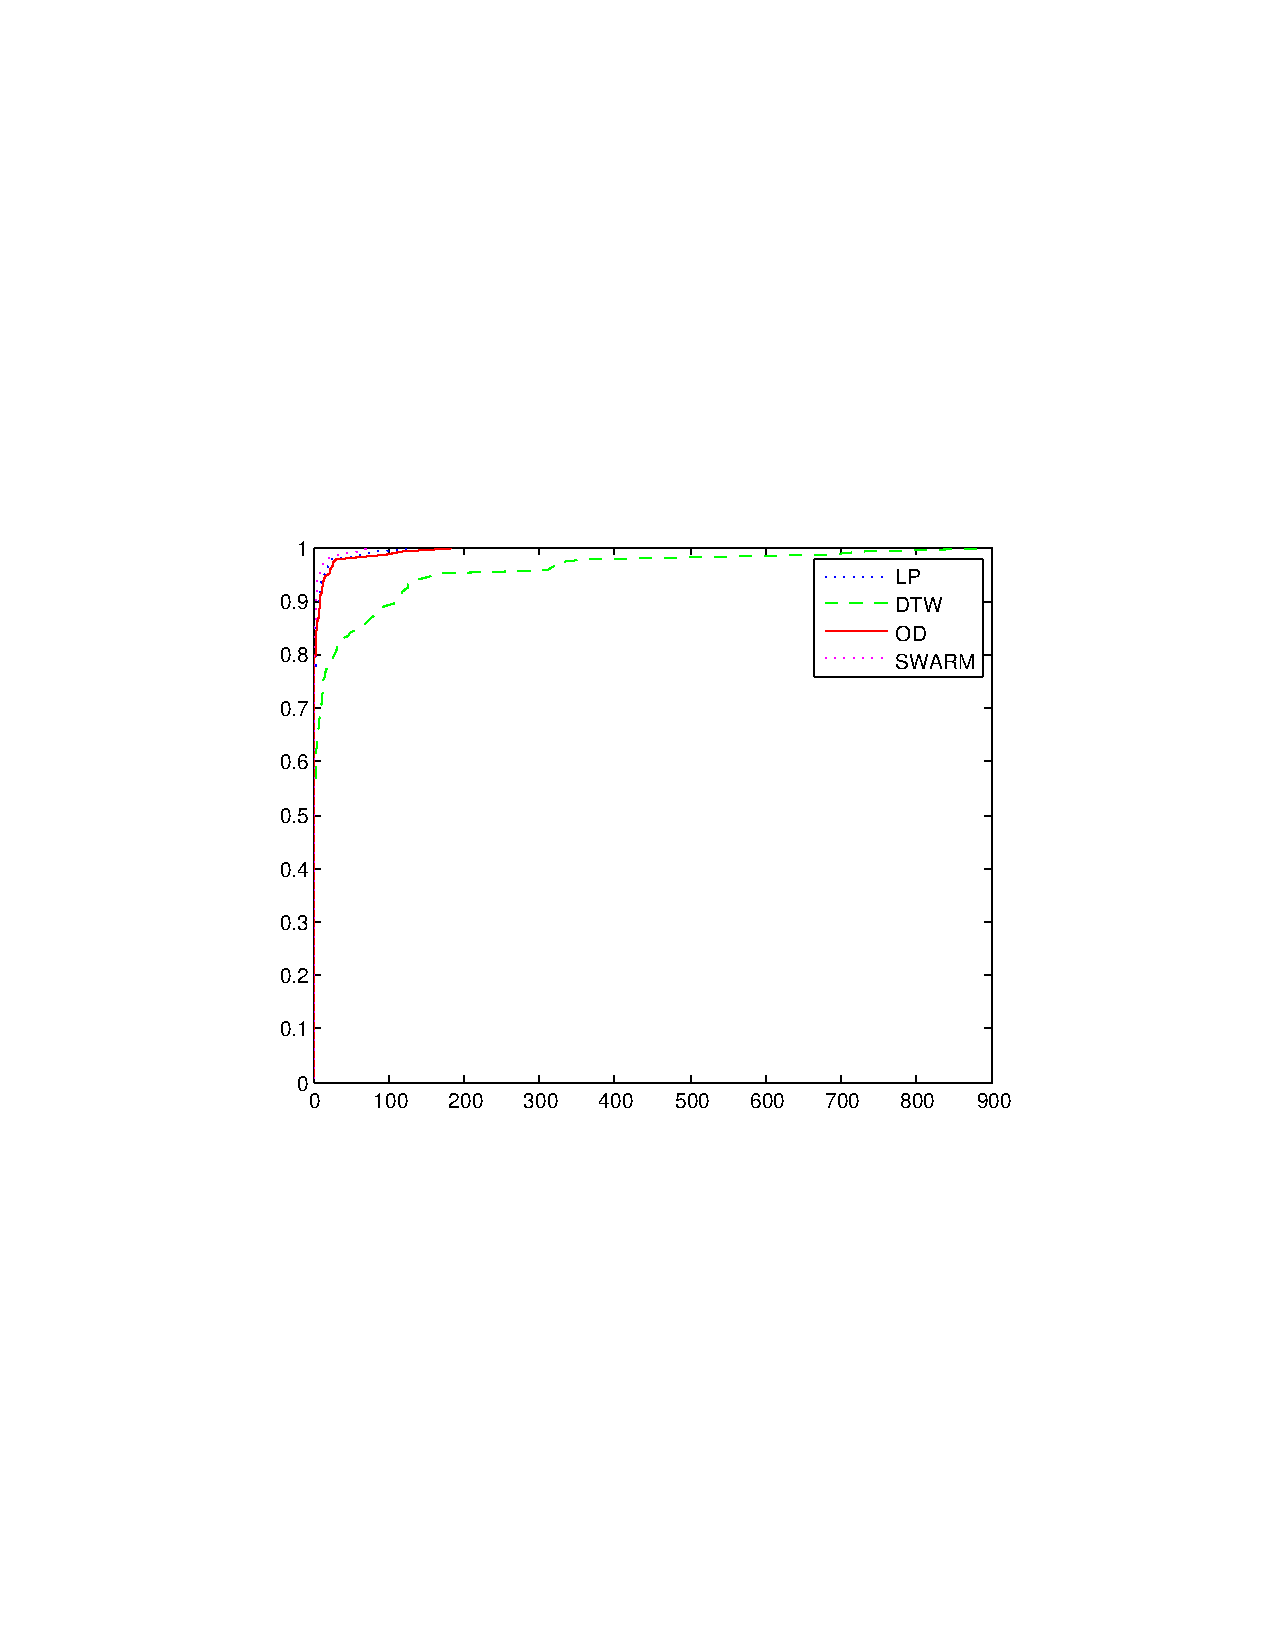
\includegraphics[scale=0.3]{figs/time_cdf.jpg}
\caption{CDF of computation time  for LP-DTW-OD}
\label{fig:time_cdf}  
\end{figure} 

\subsection{Next Location Prediction}
Another way to test the summarization of the movement patterns is to test a query trajectory and plot its predicted next location/destination as predicted by all the methods.

The next location prediction is done by the following algorithm:
\paragraph{Explanation of the algo}
For any query trajectory, resample, and compute similarity with the median trajectories of all summary clusters. Report the one with the maximum similarity. 


Let $g(i)$ be the probability of the summary $i$. Given an input traj $t_{\operatorname{in}}$, compute the distance (in meters or so) $d(i,t_{\operatorname{in}})$ between summary $i$ and $t_{\operatorname{in}}$. Now the probability that this sub-trajectory lies within summary $i$ is given by
\begin{eqnarray}
p(i,t_{\operatorname{in}}) = \frac{1}{\sqrt{2 \pi} \sigma_{t}} \mathrm{e}^{-0.5 \left( \frac{d(i,t_{\operatorname{in}})}{\sigma_{t}} \right)}
\end{eqnarray}
Here we assume that the input trajectory is a noisy input from GPS samples. $\sigma_{t}$ is the standard deviation of the sub-trajectory distance. For now take, $\sigma_{t} = \sigma_{p}$, where $\sigma_{p}$ is the standard deviation of the GPS sampling a location (value is 15.61, which is the 95-th percentile of GPS considering 30 m error). It should ideally be standard deviation introduced when we compute distance between 100 points of a path


\begin{figure}[H]
\centering   
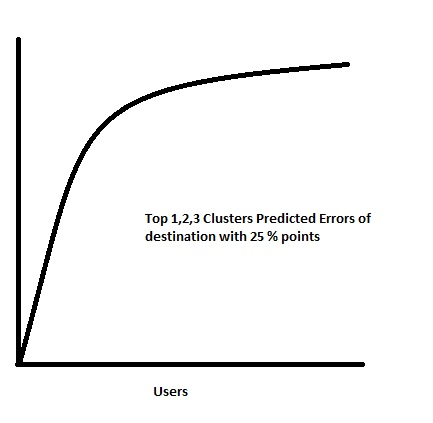
\includegraphics[scale=0.4]{figs/nextloc_10.jpg}
\caption{Destination Predicted Errors for top 1,2,3 clusters with 10 percent sample points}
\label{fig:next_loc_10}  
\end{figure} 
\begin{figure}
\centering     
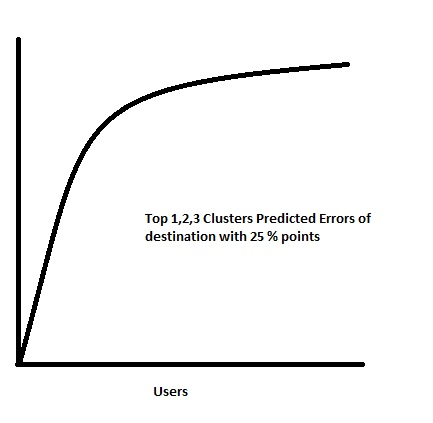
\includegraphics[scale=0.4]{figs/nextloc_25.jpg}
\caption{Destination Predicted Errors for top 1,2,3 clusters with 25 percent sample points}
\label{fig:next_loc_25}  
\end{figure} 
\begin{figure}
\centering     
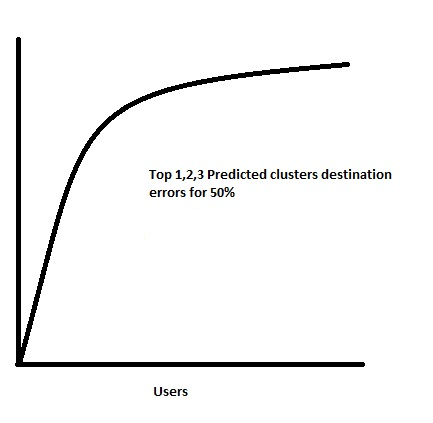
\includegraphics[scale=0.4]{figs/nextloc_50.jpg}
\caption{Destination Predicted Errors for top 1,2,3 clusters with 50 percent sample points}
\label{fig:next_loc_50}  
\end{figure} 


The best, average and worst case of prediction 
\begin{figure}[H]
\centering   
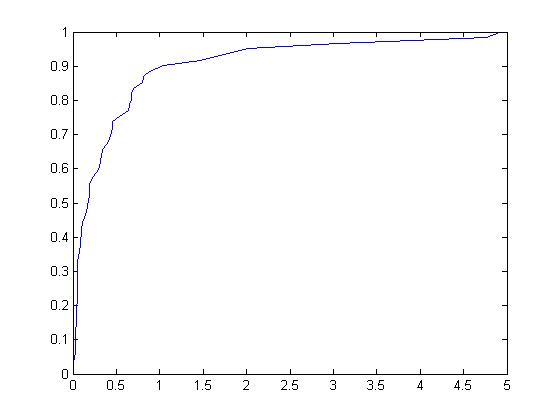
\includegraphics[scale=0.4]{figs/average_nextLoc.jpg}
\caption{Average Case of Predicted Destination}
\label{fig:average_nextLoc}  
\end{figure} 
\begin{figure}
\centering     
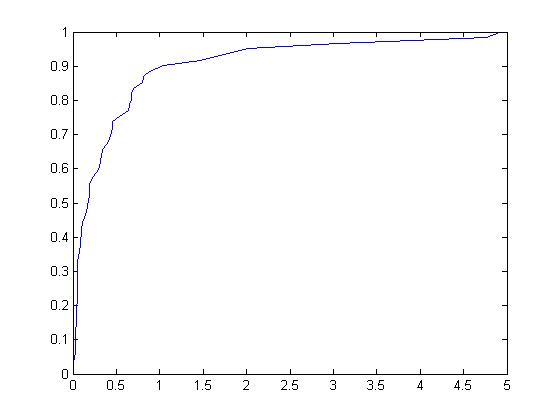
\includegraphics[scale=0.4]{figs/worst_nextLoc.jpg}
\caption{Worst Case }
\label{fig:worst_nextLoc}  
\end{figure} 
\begin{figure}
\centering     
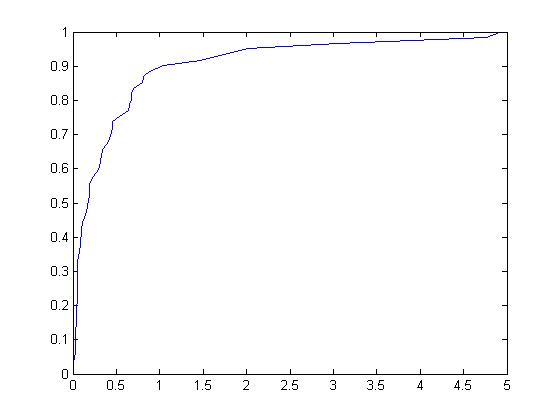
\includegraphics[scale=0.4]{figs/best_nextLoc.jpg}
\caption{Best Case}
\label{fig:best_nextLoc}  
\end{figure} 


\subsection{Visualization at various granularity }
\rednote {Remove later if needed}

\begin{figure*}
\centering   
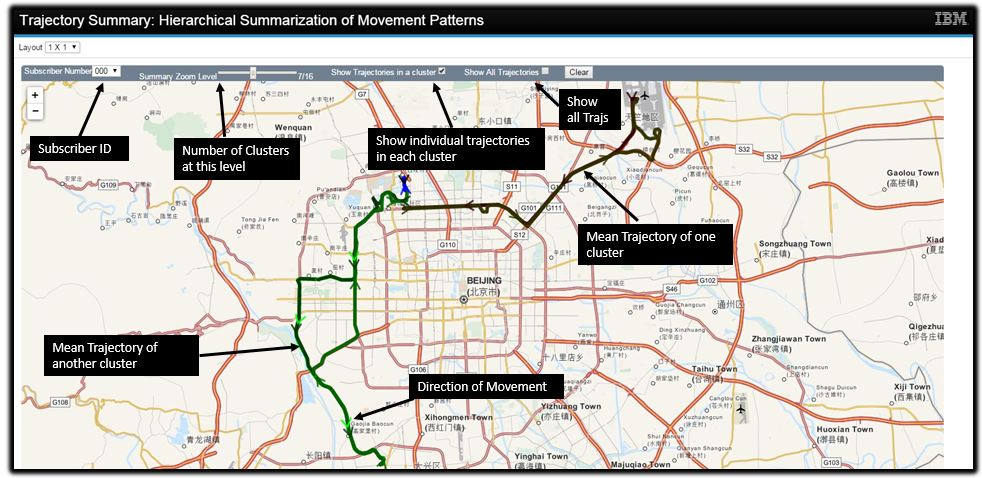
\includegraphics[scale=0.6]{figs/demo.jpg}
\caption{Visualization at various zoom levels}
\label{fig:demo}  
\end{figure*}

\subsection{Case Study: Reported Final Clusters from each method}

We take up a sample case, and show the snapshots of the final clusters as reported by all the different methods. 

\begin{figure}[H]
\centering   
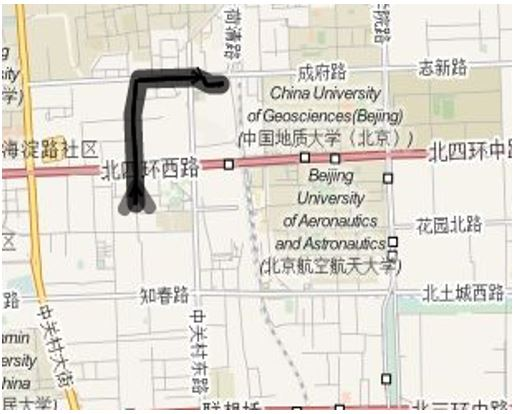
\includegraphics[scale=0.4]{figs/casestudy_dtw.jpg}
\caption{Snapshot of clusters reported by DTW}
\label{fig:casestudy_dtw}  
\end{figure} 
\begin{figure}
\centering     
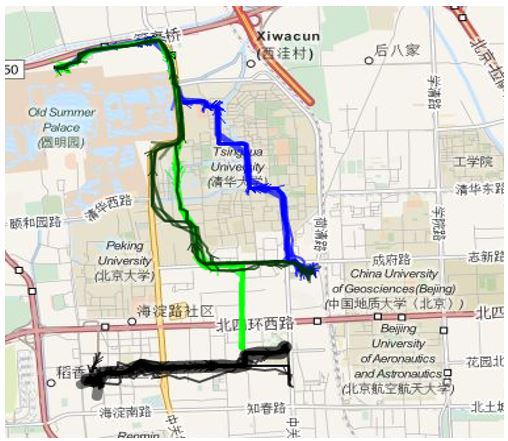
\includegraphics[scale=0.4]{figs/casestudy_swarm.jpg}
\caption{Snapshot of clusters reported by SWARM }
\label{fig:casestudy_swarm}  
\end{figure} 
\begin{figure}
\centering     
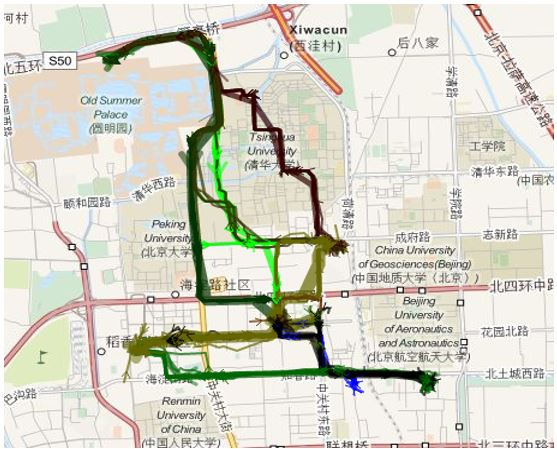
\includegraphics[scale=0.4]{figs/casestudy_our.jpg}
\caption{Snapshot of clusters reported by TrajClus-placeholder}
\label{fig:casestudy_trajclus}  
\end{figure} 
\begin{figure}
\centering     
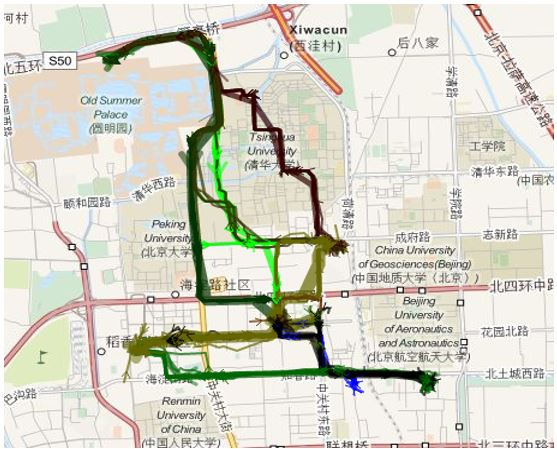
\includegraphics[scale=0.4]{figs/casestudy_our.jpg}
\caption{Snapshot of clusters reported by OD}
\label{fig:casestudy_od}  
\end{figure} 


The table below shows the statistics of the top k clusters and the number of trajectories 

\begin{table*}
	\centering
		\begin{tabular}{|c|c|c|c|c|} 
			\hline
			Method&DTW&SWARM&TrajClus&OD\\
			\hline
			Number of Clusters Reported&1&4&0&18\\
			Number of trajectories in top 3 Clusters & 5&36,15,13&0&38,37,29\\
			\hline
		\end{tabular}
	\caption{Comparison for case study}
	\label{tab:case_study}
\end{table*}